\section{Konsistenz \& Konsistenzmodelle}

\subsection{Notation}

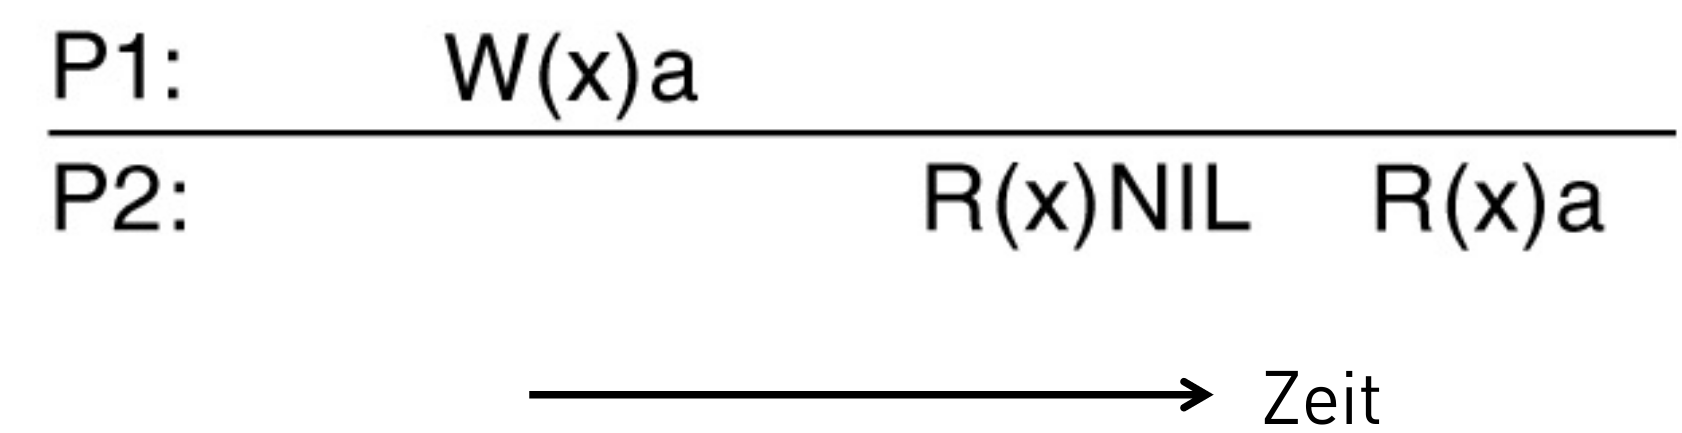
\includegraphics[height=60px]{NotationKonsistenz.png}

Im folgenden benutzen wir eine bestimmte Notation, um das Ergebnis von Schreibe- und Leseoperationen in einem verteilten System darzustellen. Wenn aus der Variable x der Wert a gelesen wurde oder in die Variable x der Wert a geschrieben wurde schreiben wir:\\

R(x)a \\
W(x)a \\

In dem oberen Diagramm bedeutet das, dass zuerst von P1 in die Variable x der Wert a geschrieben wird. Dann liest ein anderer Prozess P2 den Wert NIL (vgl. NULL) aus x. Offensichtlich ist das Ergebnis der Schreibeoperation von P1 noch nicht sichtbar. Dann liest P2 noch einmal den Wert von x und erhält nun den Wert a, d.h. offensichtlich wurde nun die Schreibeoperation mit P2 synchronisiert. Die Schreibeoperationen können jeweils auch als Nachricht betrachtet werden. Denn immer wenn auf replizierten Daten geschrieben wird bedeutet die Veröffentlichung dieses Schreibens, dass eine Nachricht an alle anderen Prozesse gesendet werden muss.

\subsection{Strikte Konsistenz}

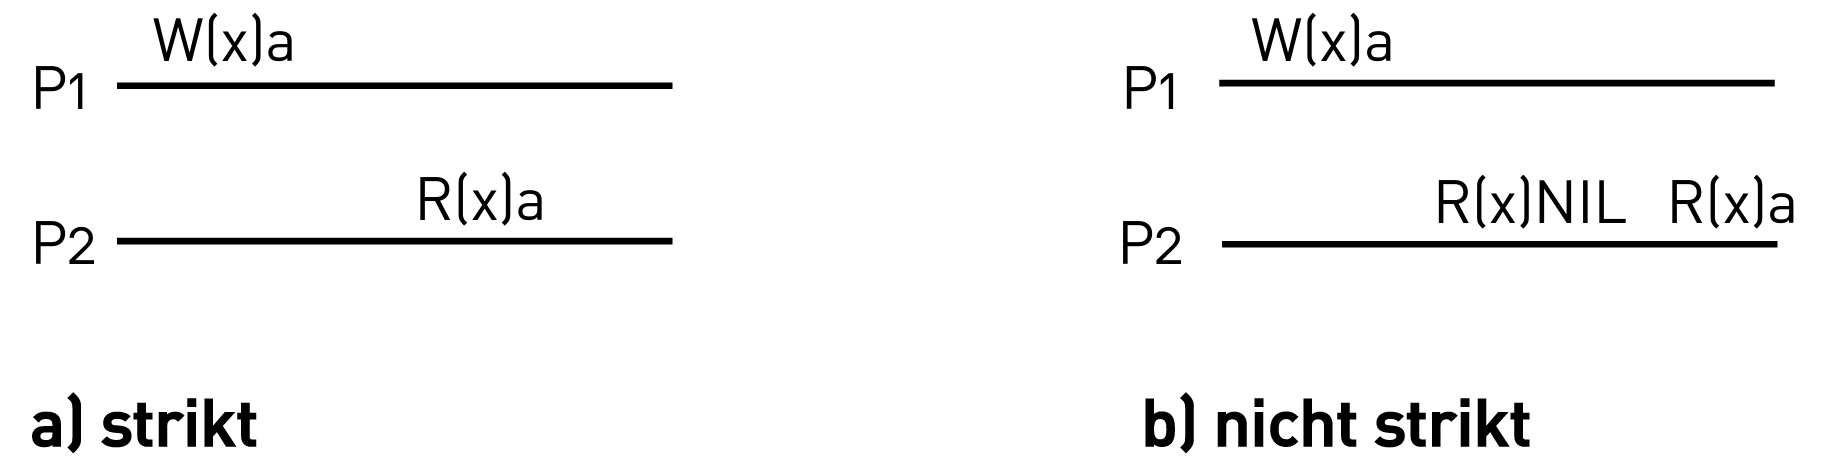
\includegraphics[height=85px]{strict-consistency.png}

Strikte Konsistenz bezeichnet, dass das Ergebnis jeder Leseoperation jeweils das Ergebnis der vorherigen Schreiboperation liefert. Strikte Konsistenz kann in einem Verteilten System nicht erreicht werden, weil die Veröffentlichung von Schreiboperationen Zeit benötigt in der das System zwangsweise inkonsistent ist.

\subsection{Sequentielle Konsistenz}

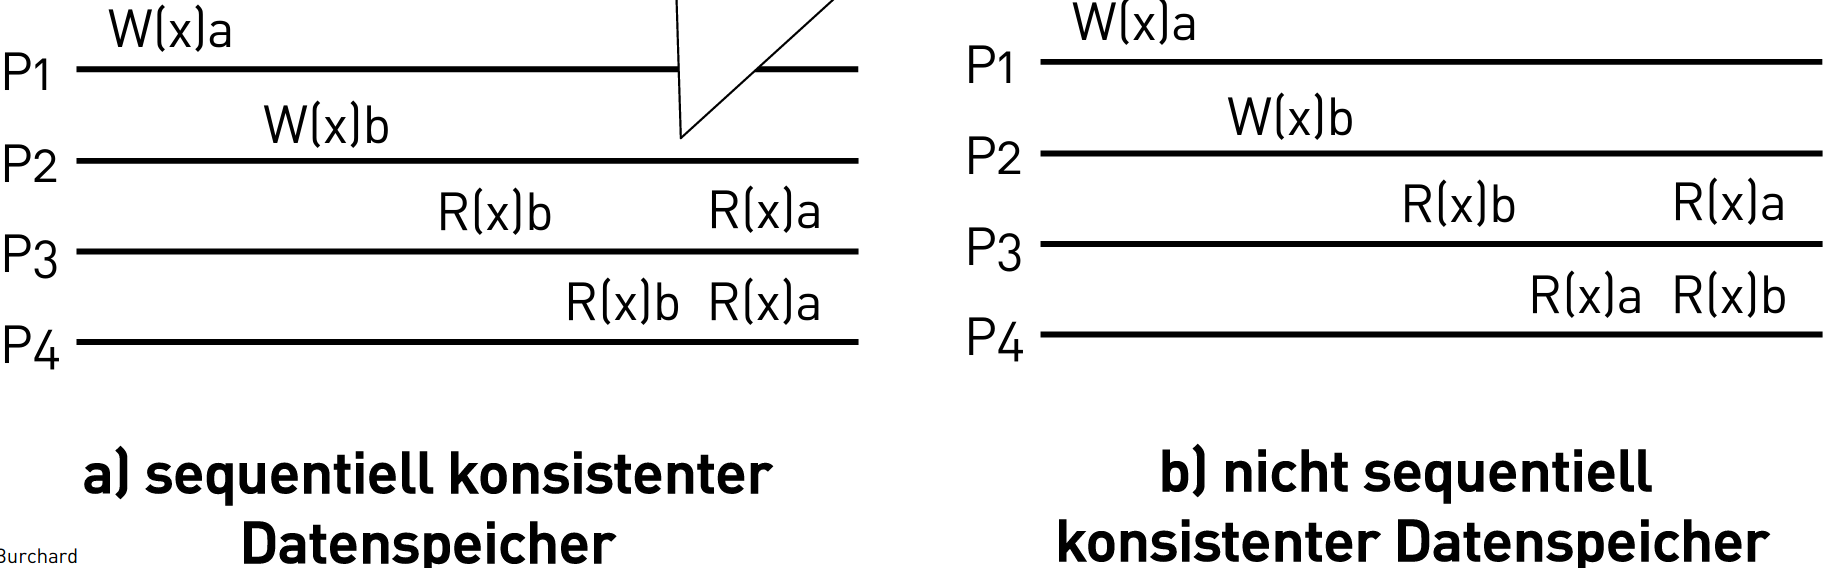
\includegraphics[height=100px]{sequential-consistency.png}

Sequentielle Konsistenz bedeutet, dass jeder Prozess bei seinen Leseoperationen die gleiche Reihenfolge von Veränderungen der Daten wahrnimmt. Nicht jeder Prozess muss jede Änderung lesen, aber wenn er sich dazu entscheidet zu lesen, dann muss die Reihenfolge der Änderungen, die gelesen werden würden, bei allen Prozessen gleich sein. \\
Dieses Konsistenzmodell lässt sich gut mit dem \hyperref[sec:master-slave]{Master-Slave-Cluster} implementieren, indem es einen Master gibt, der schreiben darf und viele Slaves, die lesen dürfen. Es gibt somit eine zentrale eindeutige Reihenfolge der Schreibeoperationen auf dem Master. Wenn zusätzlich gewährleistet wird, dass die Nachrichten, die der Master an die Slaves sendet, reihenfolgegetreu ankommen (z.B. mittels TCP), dann ist also auch gewährleistet, dass die Reihenfolge der Schreiboperationen, die auf den Slaves sichtbar ist, mit der Reihenfolge auf dem Master übereinstimmt.

\subsection{Kausale Konsistenz}

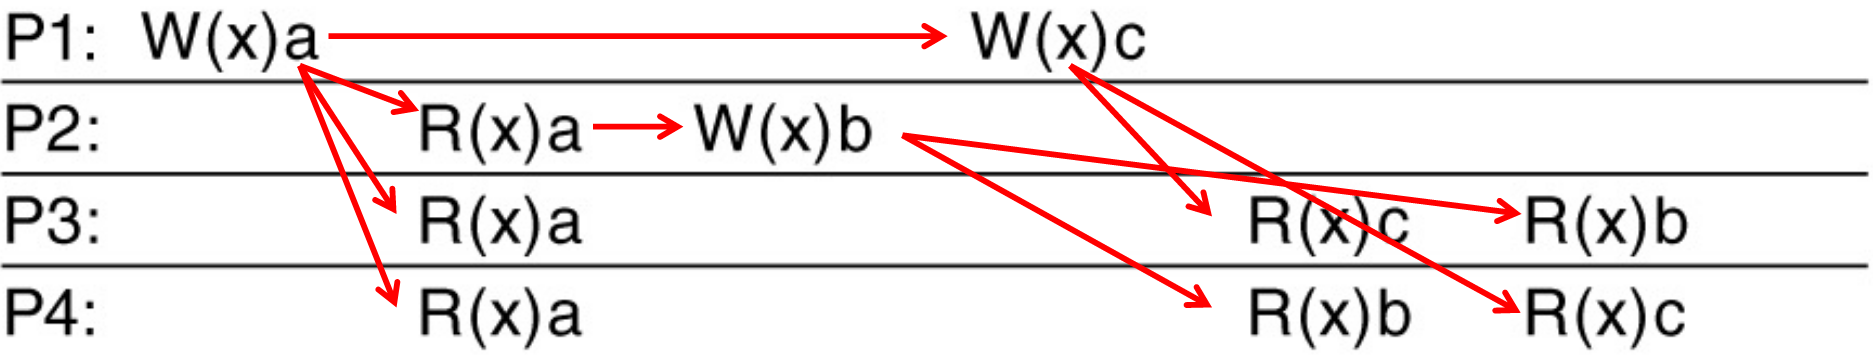
\includegraphics[height=70px]{causal-consistency-2.png}

Kausale Konstistenz ist gegeben, wenn sequentiell Konsistenz für alle Änderungen des Datenbestandes gegeben ist, die in kausalem Zusammenhang stehen könnten. Schreiboperationen $W_{1}(x)a$ und $W_{2}(y)b$ können dann in einem kausalen Zusammenhang stehen, wenn das Ergebnis von $W_{1}$ zur Zeit der Schreiboperation von $W_{2}$ bekannt ist, also wenn die Nachricht darüber, dass eine Schreiboperation stattgefunden hat, bereits erhalten wurde. Man kann sich vorstellen, dass die Schreiboperation $W_{2}$ (z.B. ein Like eines Beitrags in einem sozialen Netzwerk) nämlich nur durchgeführt worden sein könnte, weil bereits die Schreiboperation $W_{1}$ (z.B. die Veröffentlichung diese Beitrags) bekannt war. \\

In unseren Schaubildern soll ein roter Pfeil jeweils die Nachricht zeigen, welche die Änderung der Daten veröffentlicht. Jede Schreiboperation hat also $n-1$ Nachrichten zur Folge, wobei $n$ die Anzahl der Prozesse im verteilten System darstellt.\\
Im oberen Bild sehen wir also, dass ein kausaler Zusammenhang zwischen W(x)a und W(x)c, sowie zwischen W(x)a und W(x)b bestehen könnte. Es besteht allerdings kein kausaler Zusammenhang zwischen W(x)b und W(x)c. Das obere Schaubild bildet kausale Konsistenz ab, da $a \rightarrow b $ und $a \rightarrow c$ immer in dieser Reihenfolge gelesen werden. Die Reihenfolge, in der $b$ und $c$ gelesen werden, ist für die kausale Konsistenz nicht relevant und dürfte auch von verschiedenen Prozessen unterschiedlich wahrgenommen werden. \\

\subsubsection*{Implementierung kausaler Konsistenz mit Vektor-Time}

Um die kausale Konsistenz einzuhalten, muss ein Knoten beim Erhalt einer Nachricht (also einer Veröffentlichung einer Schreibeoperation) feststellen können, ob es eine Schreibeoperation gibt, von der die erhaltene Nachricht abhängen könnte, die er selbst noch nicht erhalten hat. \\
Um dies umzusetzen kann die  \hyperref[sec:vector-time]{Vektor-Time} der Nachrichten genutzt werden. Beim Erhalt einer Nachricht kann verglichen werden, ob irgendeine Komponente der Nachricht höher ist als die entsprechende Komponente der lokalen Vektor-Time. Dabei müssen aber nur die Komponenten anderer Prozesse, also nicht die des eigenen und nicht die des Senders der Nachricht, überprüft werden. Wenn dies der Fall ist, bedeutet das, dass der Absender zur Zeit des Sendens eine Nachricht von einem anderen Knoten erhalten haben muss, die der empfangene Knoten selbst noch nicht bekommen hat. Folglich ist es möglich, dass die Nachrichten in einem kausalen Zusammenhang stehen. Um kausale Konsistenz zu erreichen darf die Änderung an den eigenen Daten also erst sichbar werden, wenn die Nachricht(en), mit denen sie in kausalem Zusammenhang steht, auch eingetroffen sind. Falls also in der Zwischenzeit eine Schreiboperation (hier die in grau dargestellte) angefordert wird, so muss sie verzögert werden.

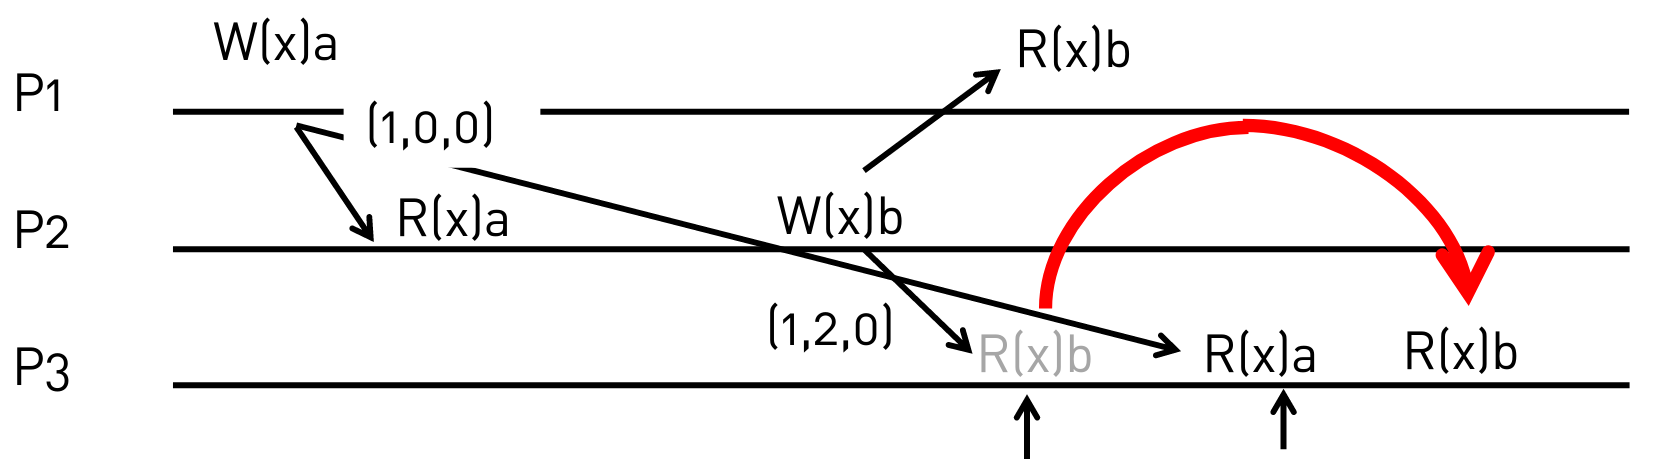
\includegraphics[height=90px]{causal-consistency-3.png}


\subsection{Urbildbasierte Protokolle}

Urbildbasierte Protokolle sind solche, die zu jeder Zeit nur genau einen Prozess des verteilten Systems schreiben lassen und dadurch sequentielle Konsistenz erreichen. Eine Implementierung ist das \hyperref[sec:master-slave]{Master-Slave-Cluster} mit einem Schreiber und vielen Lesern. Hierbei gibt es 2 grundlegende Weisen, wie man Schreibeoperationen umsetzen kann, die im Folgenden kurz beleuchtet werden sollen.

\subsubsection{Entferntes Schreiben}

Beim entfernten Schreiben werden Schreibeanfragen eines Slaves an den Server weitergeleitet, der diese dann durchführt.

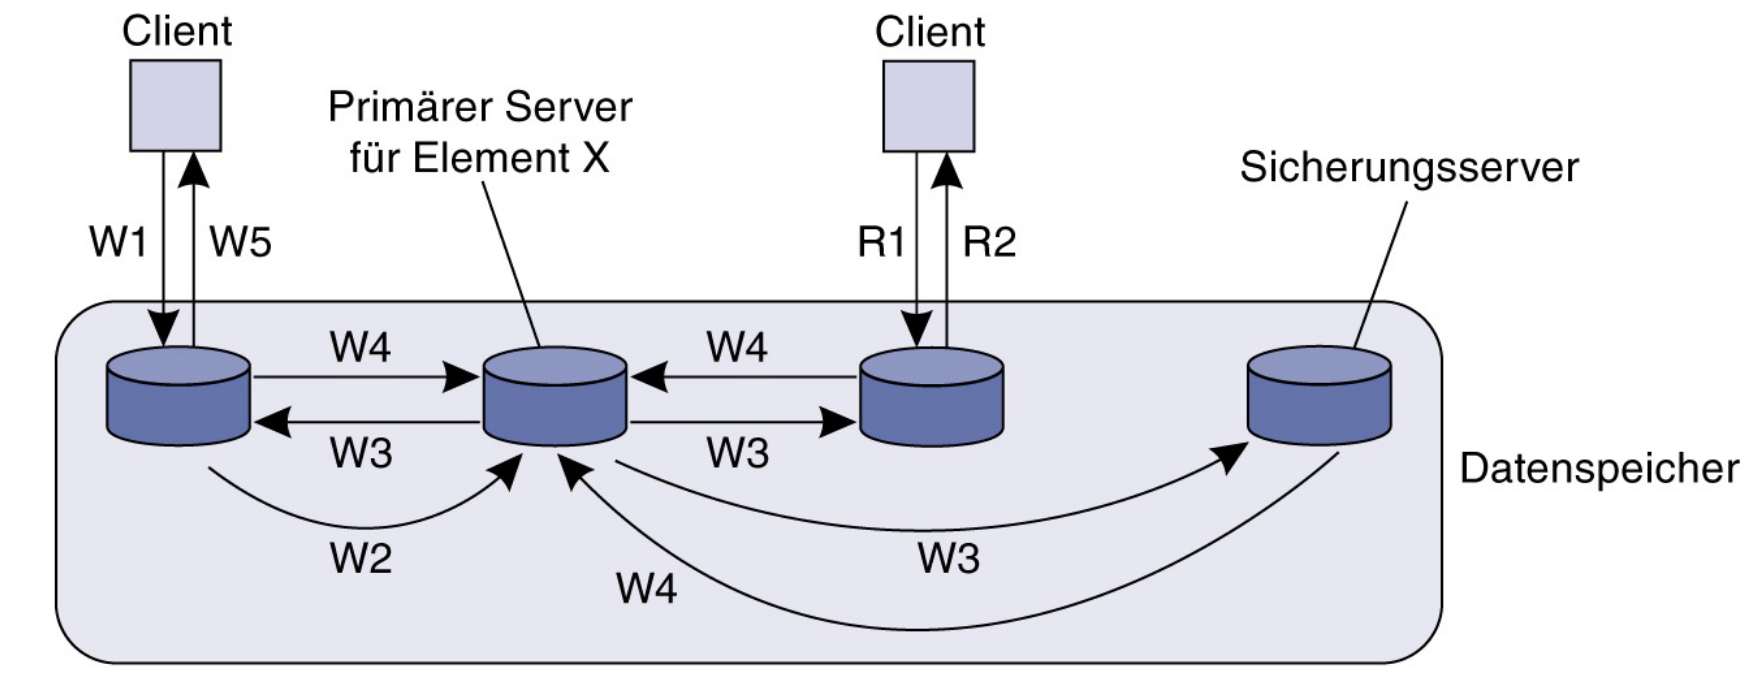
\includegraphics[height=150px]{entferntes-schreiben.png}

\subsubsection{Lokales Schreiben}

Beim lokalen Schreiben wird zunächst die benötigte Ressource vom Master auf einen Slave kopiert, sodass dieser den aktuellsten Stand dieser Ressource hat. Dann wird dieser Slave zum Master ernannt und die Schreiboperation kann direkt lokal ausgeführt werden. Diese Variante erfordert mehr Logik und Aufwand für das Kopieren. Allerdings kann sie performanter sein, wenn ein Client in der Regel sehr viele Daten schreibt. In diesem Fall werden nämlich viele Nachrichten über das Netzwerk vermieden.

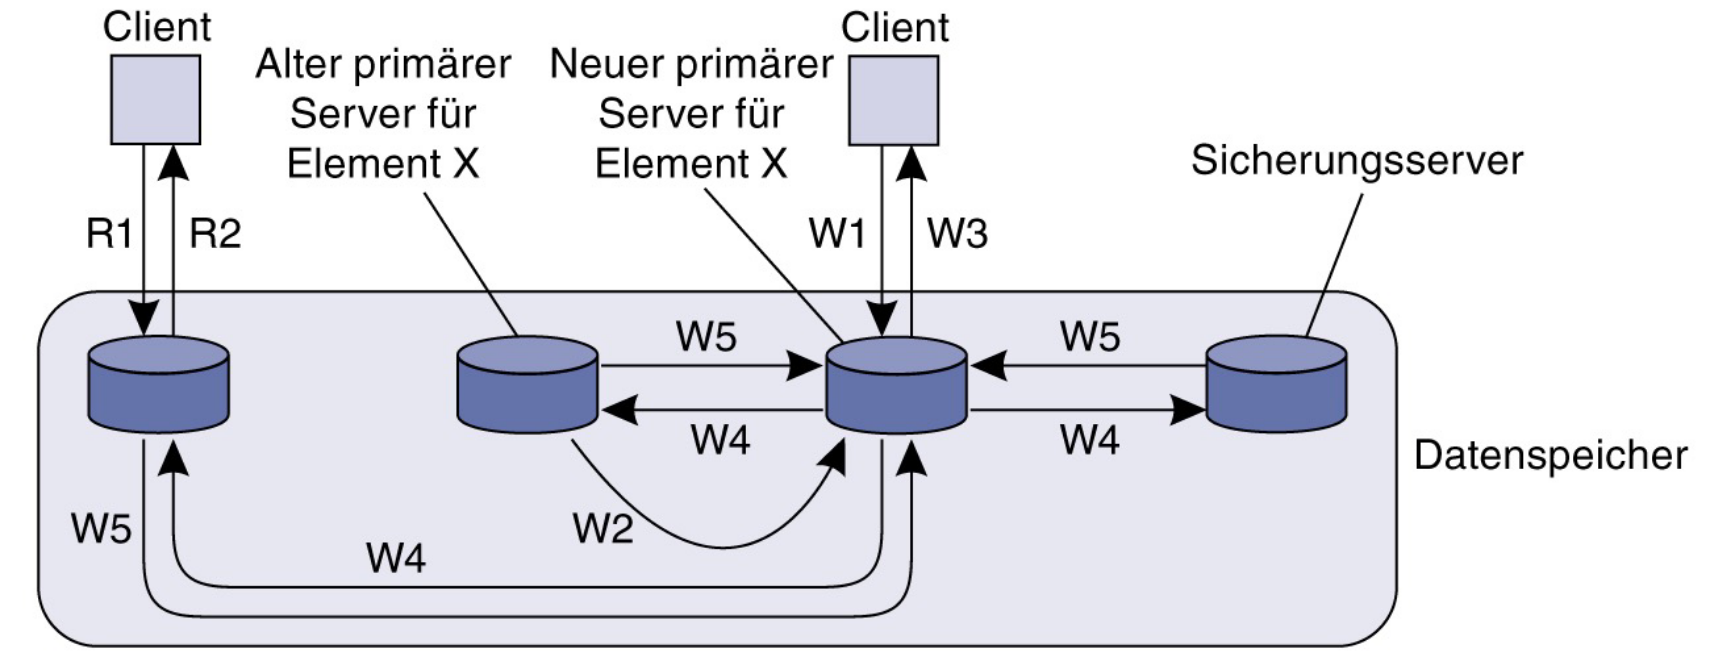
\includegraphics[height=150px]{lokalesSchreiben.png}


\subsection{Transaktionsbasierte Protokolle}

\subsection{Prinzip von Transaktionen}

Transaktionen werden so aufgefasst, dass für eine Menge von schreibenden Operationen, die als Transaktion zusammengefasst werden, die ACID Prinzipien gelten, wie man sie von Datenbanken kennt:
\begin{itemize}
      \item \textbf{A}tomicity
      \item \textbf{C}onsistency
      \item \textbf{I}solation
      \item \textbf{D}urability
\end{itemize}

In einem verteilten System wird die Schwierigkeit erhöht, da verlangt wird, dass auf einer bestimmten Menge von Remote-Rechnern eine Transaktion durchgeführt werden soll.

\subsubsection{2-Phasen-Commit}
\label{sec:2pc}
Der 2-Phasen-Commit, kurz 2PC, ist ein Protokoll, dass gewährleisten soll, dass eine Transaktion auf allen oder auf keinem Rechner aus einer Menge von Remote-Rechnern durchgeführt wird. Führt also ein Rechner lokal ein ABORT aus, so sollen andere Rechner auch einen ABORT ausführen, der ABORT soll also global gelten. Ein globaler COMMIT gelingt genau dann, wenn er bei jedem Rechner lokal gelingt.\\

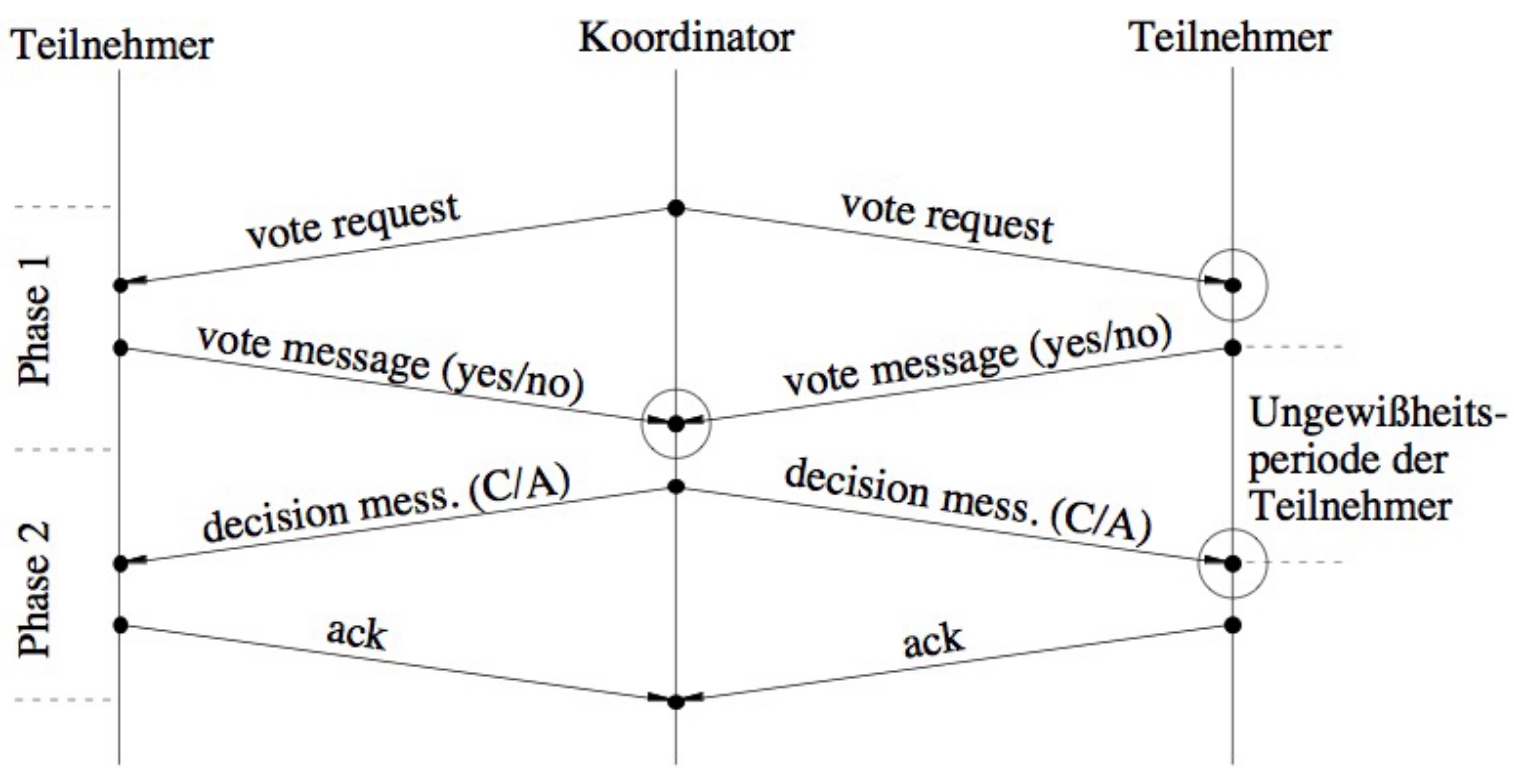
\includegraphics[height=200px]{2pc-nachrichtenfluss.png}

In 2PC haben wir einen lokalen Koordinator und $n$ Teilnehmer. Der Koordinator macht die globalen Entscheidungen über ABORT und COMMIT und kommuniziert sie mit allen Teilnehmern. Das System ist also im Sinne eines Master-Slave-Clusters aufgebaut, dass den Koordinator als schreibende Einheit hat. In dem Beispielbild gehen wir davon aus, dass die Transaktion bereits vom Koordinator begonnen wurde und er auch schon fertig mit Schreiben ist, da der eigentlich spannende Teil natürlich der COMMIT ist.\\
Damit der Koordinator eine Entscheidung treffen kann, sodass die oben gestellten Forderungen gelten, muss er, bevor er einen globalen COMMIT verkündet, sicher sein, dass alle Rechner diesen COMMIT auch durchführen können. Deshalb sendet er zunächst einen Vote-request an alle Teilnehmer. Die Teilnehmer antworten darauf mit der Information, ob sie den COMMIT in der Zukunft auf jeden Fall durchführen können oder nicht. Wenn die Antwort von allen Knoten eingetroffen ist kann der Koordinator die Entscheidung treffen, die er allen Teilnehmern sendet. Diese Führen dann die Operation, also COMMIT oder ABORT lokal aus.\\
Man kann das Verfahren auch als State-Machine visualisieren:

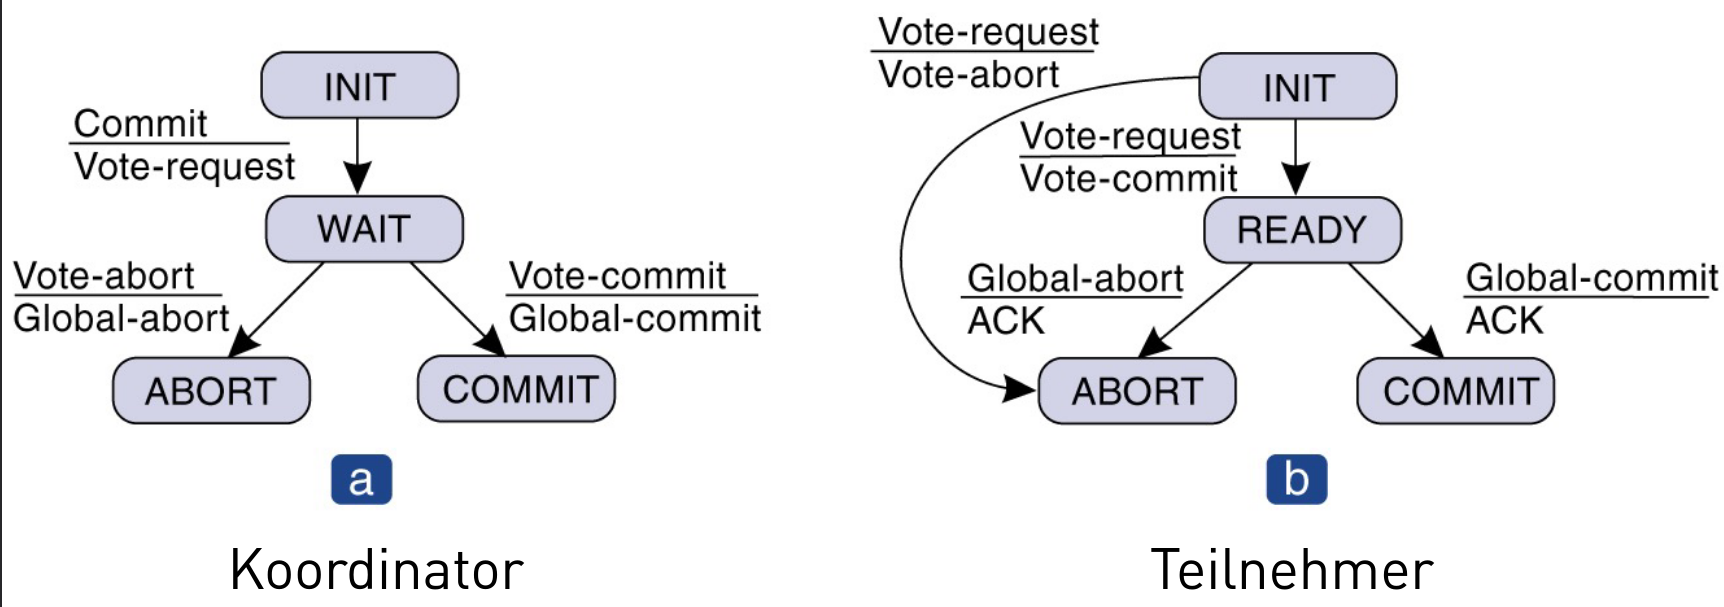
\includegraphics[height=150px]{2pc-state-machine.png}

Das 2PC-Protokoll hat aber Probleme bezüglich Fehlertoleranz. In der Zeit in der ein Teilnehmer schon mit einer Vote Message abgestimmt hat, aber noch keine Antwort über das Ergebnis vom Koordinator erhalten hat, ist er nicht handlungsfähig. Er darf weder die Transaktion ABORTen, da er schon zugesagt hat, dass er sie in der Zukunft COMMITen könnte, noch darf er sie COMMITen, da er noch kein grünes Licht vom Koordinator bekommen hat. Damit ein Teilnehmer nicht ewig in solch einem Zustand verweilt, ist es sinnvoll einen Timout zu setzen. Die Frage ist nur, was der Teilnehmer machen soll, wenn es zu einem Timeout kommt. Die Antwort auf diese Frage liefert das Terminierungsprotokoll.\\
Laut dem \textbf{Terminierungsprotokoll} soll ein Teilnehmer bei einem Timeout einen anderen Knoten q um Hilfe fragen. Es gibt 3 Möglichkeiten wie q antworten kann:
\begin{enumerate}
      \item q hat die Entscheidung des Koordinators bereits erhalten und gibt sie an den Fragenden weiter
      \item q hat selbst noch kein Vote abgegeben und kann daher für ABORT voten, um dafür zu sorgen, dass die globale Entscheidung ein ABORT wird
      \item q befindet sich auch im wartenden Zustand und kann nicht helfen
\end{enumerate}

Kritisch ist der dritte Fall, für den es tatsächlich keine Lösung gibt.\\

Außerdem sollten wir uns über \textbf{Crash Recovery} Gedanken machen, also über die Frage was ein Rechner tun soll, wenn er nach einem Ausfall wieder online ist. Die Lösung ist jeden Zustandsübergang auf die Festplatte zu schreiben, sodass bei der Recovery die Information von dort genutzt werden kann, um fortzufahren.\\

Obwohl das 2PC-Protokoll scheitert, wenn alle Rechner in einem wartenden Zustand sind, also das Terminierungsprotokoll nicht erfolgreich ist, ist es dennoch praktisch einsetzbar, falls genau solch ein Zustand anderweitig verhindert werden kann. Zum Beispiel in Datacentern, in denen es selten vorkommt, dass Rechner nicht erreichbar sind, ist eine Vermeidung dieses Fehlerzustands mit statistisch hoher Wahrscheinlichkeit gegeben.

\subsubsection{Quoren}
\label{sec:quorums}

Die Idee von Quoren ist, dass wir nicht gewährleisten müssen, dass alle Rechner des Clusters eine Transaktion committen. Stattdessen können wir verlangen, dass bloß mindestens eine Teilmenge der Rechner die Transaktion committen und wir beim Lesen sicherstellen, dass wir die Information von einem dieser Rechner erhalten.\\

Um das zu gewährleisten definieren wir folgende Quoren (minimale Anzahl für die Durchführung einer Operation) bei $n$ Teilnehmern:
\begin{enumerate}
      \item Schreibquorum QW $> \frac{n}{2}$
      \item Lesequorum QR mit $QR + QW > n$
\end{enumerate}

Um eine Operation global durchzuführen, muss sie also auf mindestens so vielen Teilnehmern des Rechnernetzes durchgeführt werden, wie wir im Quorum festgelegt haben. Mit der ersten Bedingung stellen wir sicher, dass es nicht mehrere parallele Schreiboperationen geben darf. Mit der zweiten Bedingung stellen wir sicher, dass beim Lesen von Daten für jeden Datensatz mindestens einer der antwortenden Rechner die aktuellste Version zu diesem Datensatz zurückliefert. Das liegt daran, dass durch die beiden Quoren gewährleistet ist, dass die Menge der lesenden Rechner und die Menge der schreibenden Rechner für jede Transaktion nicht disjunkt sind. Nun muss man nur noch herausfinden, welches der gelesenen Replikate das aktuellste ist. Das kann mithilfe von \hyperref[sec:logic-time]{logischer Zeit} erreicht werden.\\

Bei der Benutzung von Quoren muss es nicht zwangsläufig einen Koordinator geben, d.h. das System kann so designed werden, dass jeder Knoten schreiben darf. In diesem Fall kann es zu Deadlocks kommen, wenn ein Rechner, der eine Schreibanfrage stellt und schon einige Rechner für das Schreiben allokiert hat, so lange wartet, bis er genug Rechner allokieren kann und das Quorum erreicht ist und gleiches parallel von einem anderen Rechner getan wird. Allerdings kann dies leicht mit Timeouts gelöst werden, bei deren Auftritt nach einem zufälligen Zeitintervall ein erneuter Versuch gestartet wird.\\

Abschließend lässt sich sagen, dass Quoren den Aufwand beim Schreiben verringern, aber den Aufwand beim Lesen vergrößern, da nun nicht mehr nur von einem einzigen Rechner, sondern von mehreren gelesen werden muss.

\subsubsection{Fehlerbehandlung}

Es gibt verschiedene Arten, wie wir in einem verteilten System mit dem versenden von Nachrichten, bzw. mit Schreibeoperationen umgehen können, die wir Fehlersemantiken nennen:

\begin{enumerate}
      \item \textbf{Maybe:}\\
            Eine Nachricht wird genau einmal versendet und es gibt keine Fehlerbehandlung
      \item \textbf{At-most-once:}\\
            Falls ein Fehler auftritt versenden wir die Nachricht erneut. Allerdings stellen wir sicher, dass das Duplikate der Nachricht auf dem Server erkannt werden, sodass die Nachricht effektiv nur einmal eintritt. \textit{At-least} bedeutet, dass es vorkommen kann, dass auch bei mehrmaligem erneuten Versuchen der Server nicht erreicht werden kann.
      \item \textbf{At-least-once:}\\
            Eine Nachricht wird so oft gesendet, bis sie ankommt. Es werden keine Duplikate herausgefiltert. Daher ist diese Methode nur für idempodente Operationen sinnvoll.
      \item \textbf{Exactly-once:}\\
            Es wird sichergestellt, das die Anfrage genau einmal vom Server bearbeitet wird. In der Praxis ist es nicht möglich das vollständig zu ermöglichen. Es sollte daher geklärt werden, was in einer konkreten Implementierung dieser Fehlersemantik gewährleistet wird. In der Regel läuft es darauf hinaus, dass diese Fehlersemantik eigentlich hätte \textit{at-most-once} genannt werden sollen.
\end{enumerate}

Wir wollen uns nun überlegen, was sinnvoll wäre, um eine \textbf{at-most-once} Fehlersemantik zu implementieren. Die Fehlersituation, die wir dazu im Folgenden betrachten wollen ist folgende:
\begin{enumerate}
      \item Ein Client hat eine Anfrage für eine Schreiboperation an einen Server gesendet. Dann hat er nach einiger Zeit keine Reaktion vom Server erhalten und reagiert mit einem Timeout.
      \item Der Client sendet die Anfrage erneut
      \item Durch eine eindeutige ID ist gekennzeichnet, dass die beiden Nachrichten des Clients zur selben Operation gehören
\end{enumerate}

Diese Situation kann verschiedene Ursachen haben, bei denen es verschiedene Dinge zu beachten gilt:
\begin{itemize}
      \item Die Request-Nachricht des Clients ging im Netzwerk verloren:\\
            In diesem Fall kann genau die selbe Nachricht nocheinmal gesendet werden, da dieser Zustand äquivalent zum Zustand vor dem ersten Senden der Nachricht ist.
      \item Serverabsturz:\\
            Verhält sich wie 1.
      \item Die Response-Nachricht des Servers (z.B. ein ACK) ging im Netzwerk verloren:\\
            In diesem Fall muss der Server erkennen, dass die Nachricht bereits verarbeitet wurde und sollte die angefragte Operation nicht erneut durchführen. Die Antwort ist möglicherweise noch gecached und kann demnach von dort direkt entnommen werden.
      \item Der Server ist zwar online, aber so langsam, dass das Timout entsteht:\\
            In diesem Fall ist eine Prävention des Timeouts sinnvoll, indem der Server eine vorläufige Antwort schickt, die suggeriert, dass die tatsächliche Antwort mit Verzögerung gesendet werden wird.
\end{itemize}